\documentclass{IEEEcsmag}

\usepackage[colorlinks,urlcolor=blue,linkcolor=blue,citecolor=blue]{hyperref}

\usepackage{upmath}
\usepackage{url}
\usepackage{breakurl}
% \usepackage[breaklinks]{hyperref}
% \def\UrlBreaks{\do\/\do-}

\jvol{Vol. 2}
\jnum{CS 611}
\paper{8}
\jmonth{December}
\jname{THREADS}
\pubyear{2023}
\newtheorem{theorem}{Theorem}
\newtheorem{lemma}{Lemma}

\setcounter{secnumdepth}{0}

\begin{document}
\setcounter{page}{1}
\title{The Shape of Information}

\author{Tyler Trogden}
\affil{Brigham Young University}

\markboth{The Shape of Information}{}

\begin{abstract}
\end{abstract}

\maketitle

\chapterinitial{}


\section{SECTIONS}


\section{CONCLUSION}



\section{ACKNOWLEDGMENT}
I'd like to acknowledge that I hate writing about things that I care absolutely nothing
about. Thank you.

\bibliographystyle{ieeetr}
\bibliography{refs}

\begin{wrapfigure}{l}{0.16\textwidth}
  \centering
  \vspace{-5mm}
  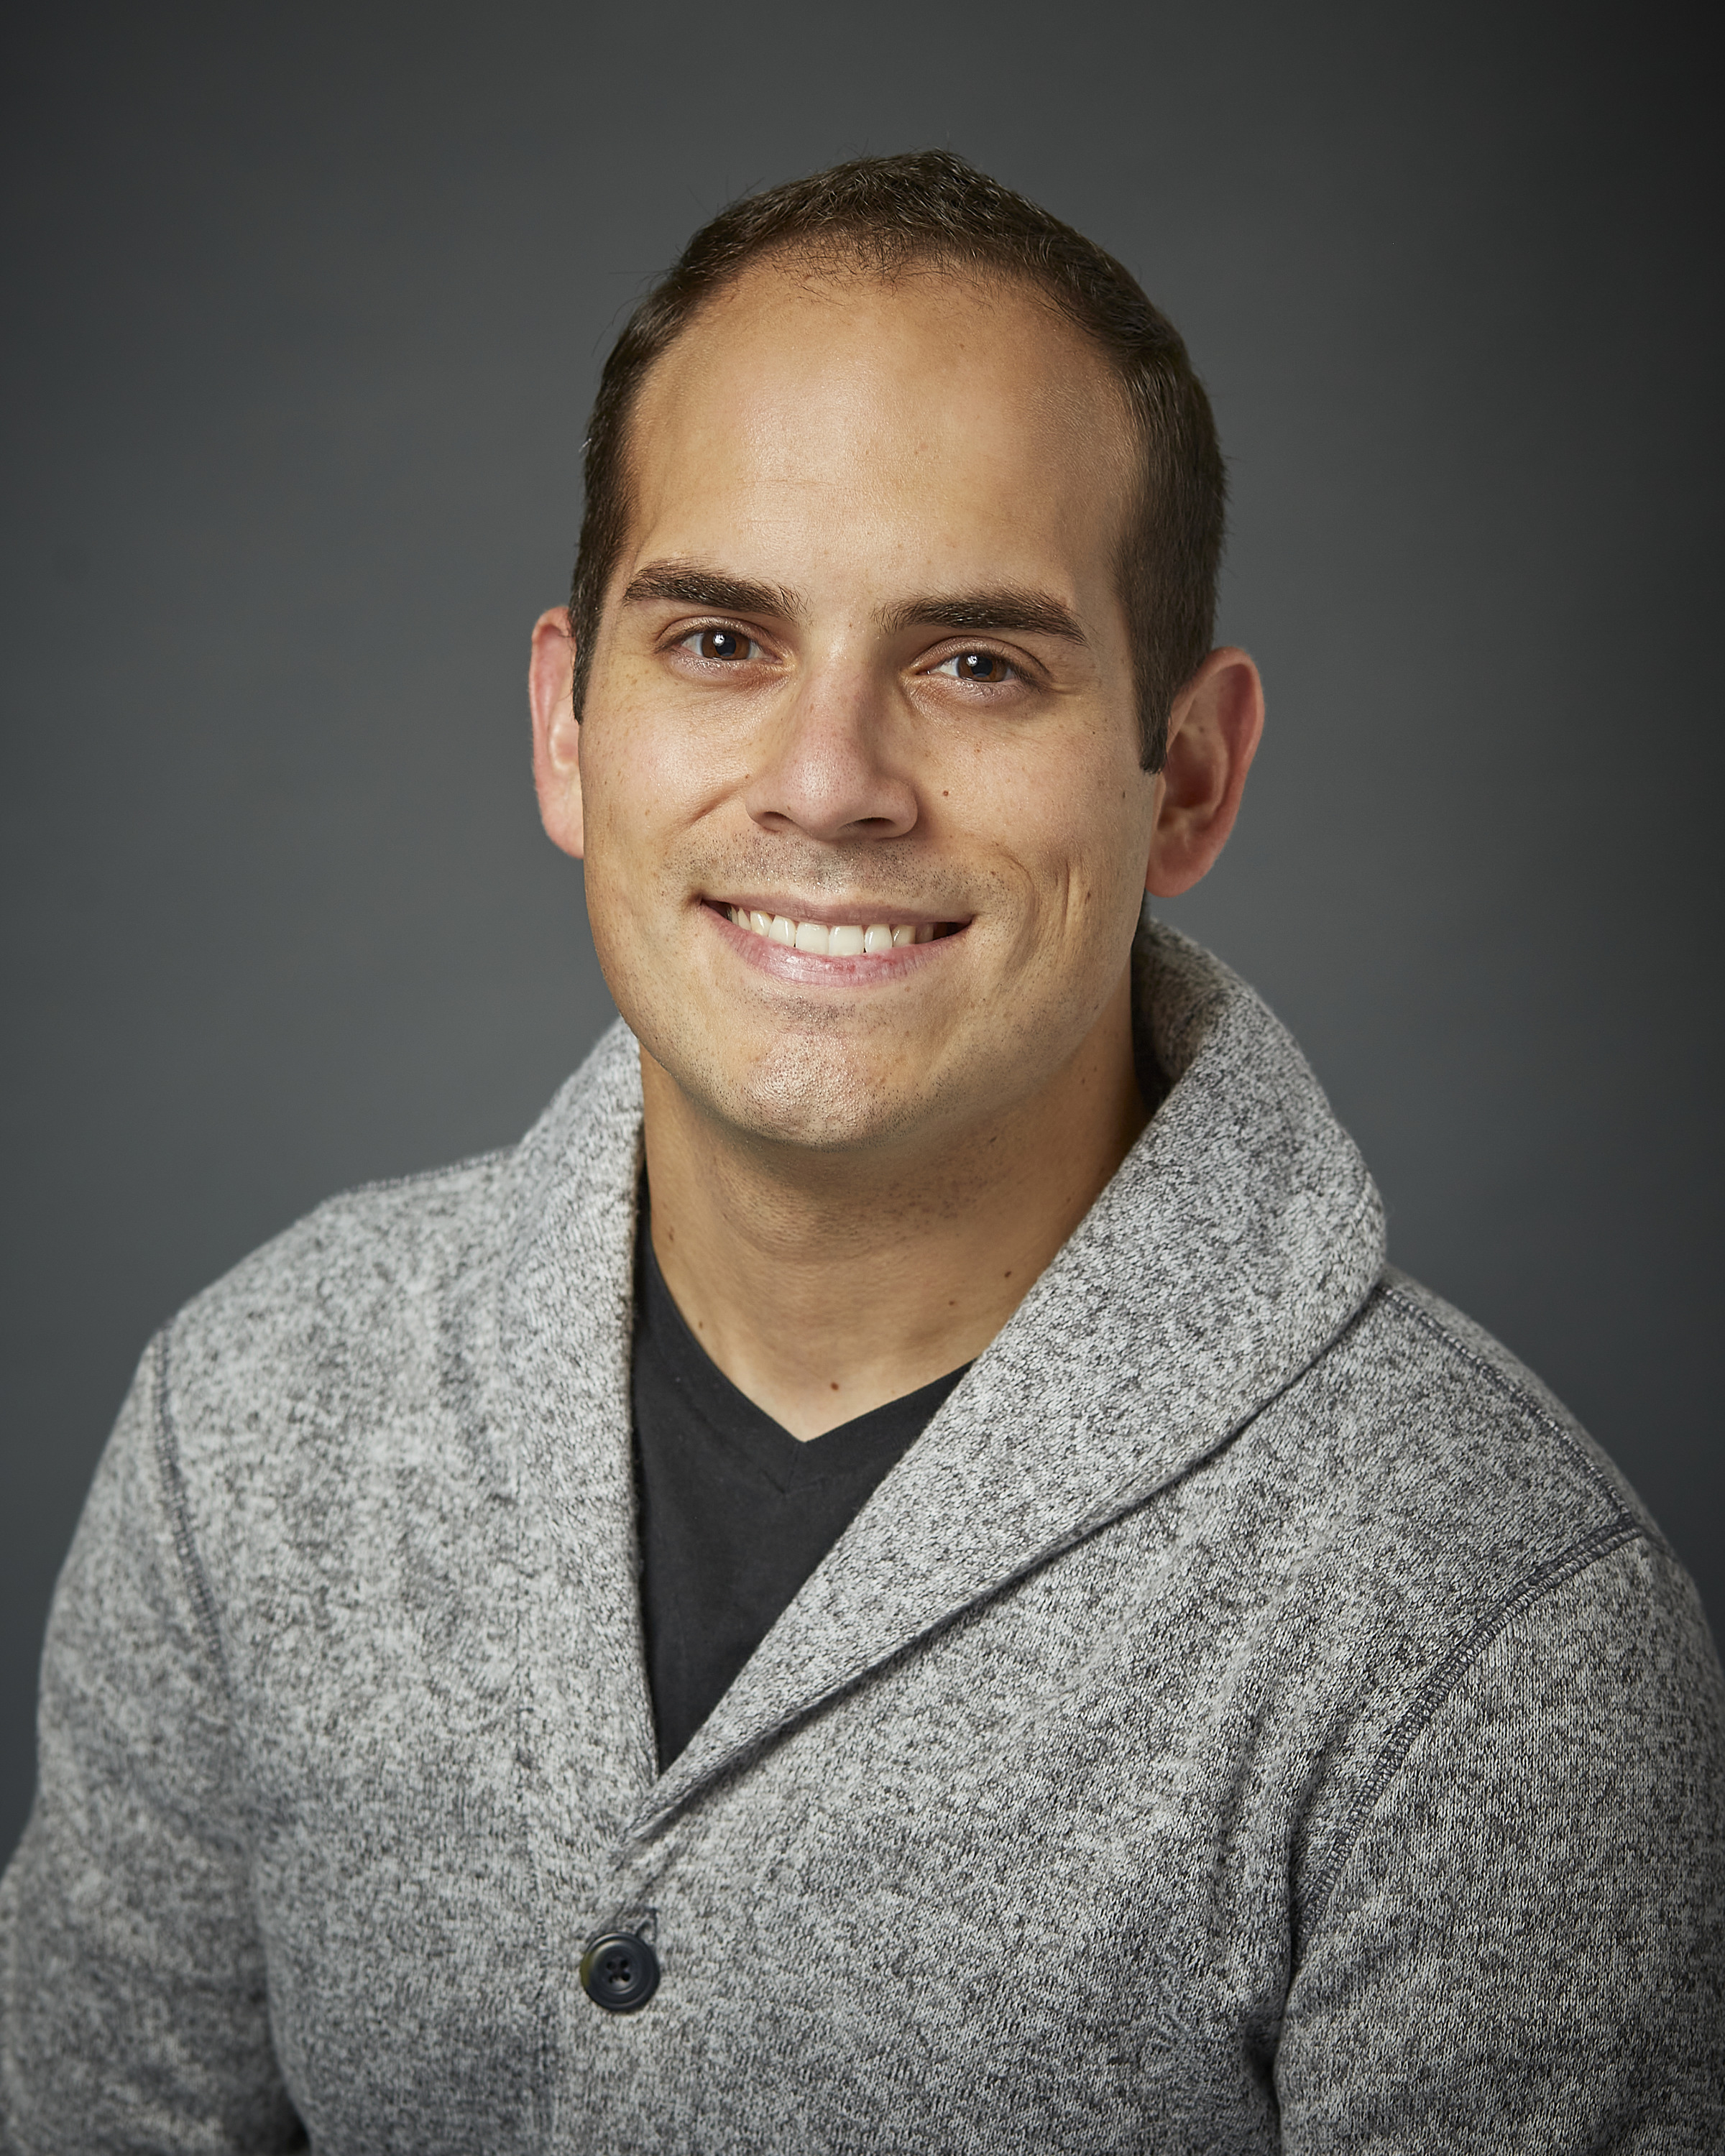
\includegraphics[width=0.18\textwidth]{portrait.jpg}
  \end{wrapfigure}\begin{IEEEbiography}{Tyler Trogden} is a Ph.D. candidate 
in Computer Science at BYU performing research in the field of machine learning
and AI.
\end{IEEEbiography}

\end{document}